\documentclass{article}

\usepackage{graphicx}
\usepackage{tikz}
\usepackage{tikzsymbols}
\usetikzlibrary{calc,patterns,shapes.geometric}
\pagestyle{empty}
\usepackage[margin=0pt]{geometry}
\geometry{papersize={14in,12in}}

\def\centerarc[#1](#2)(#3:#4:#5){\draw[#1] ($(#2)+({#5*cos(#3)},{#5*sin(#3)})$) arc (#3:#4:#5);}

\begin{document}
	\begin{figure}
		\centering
		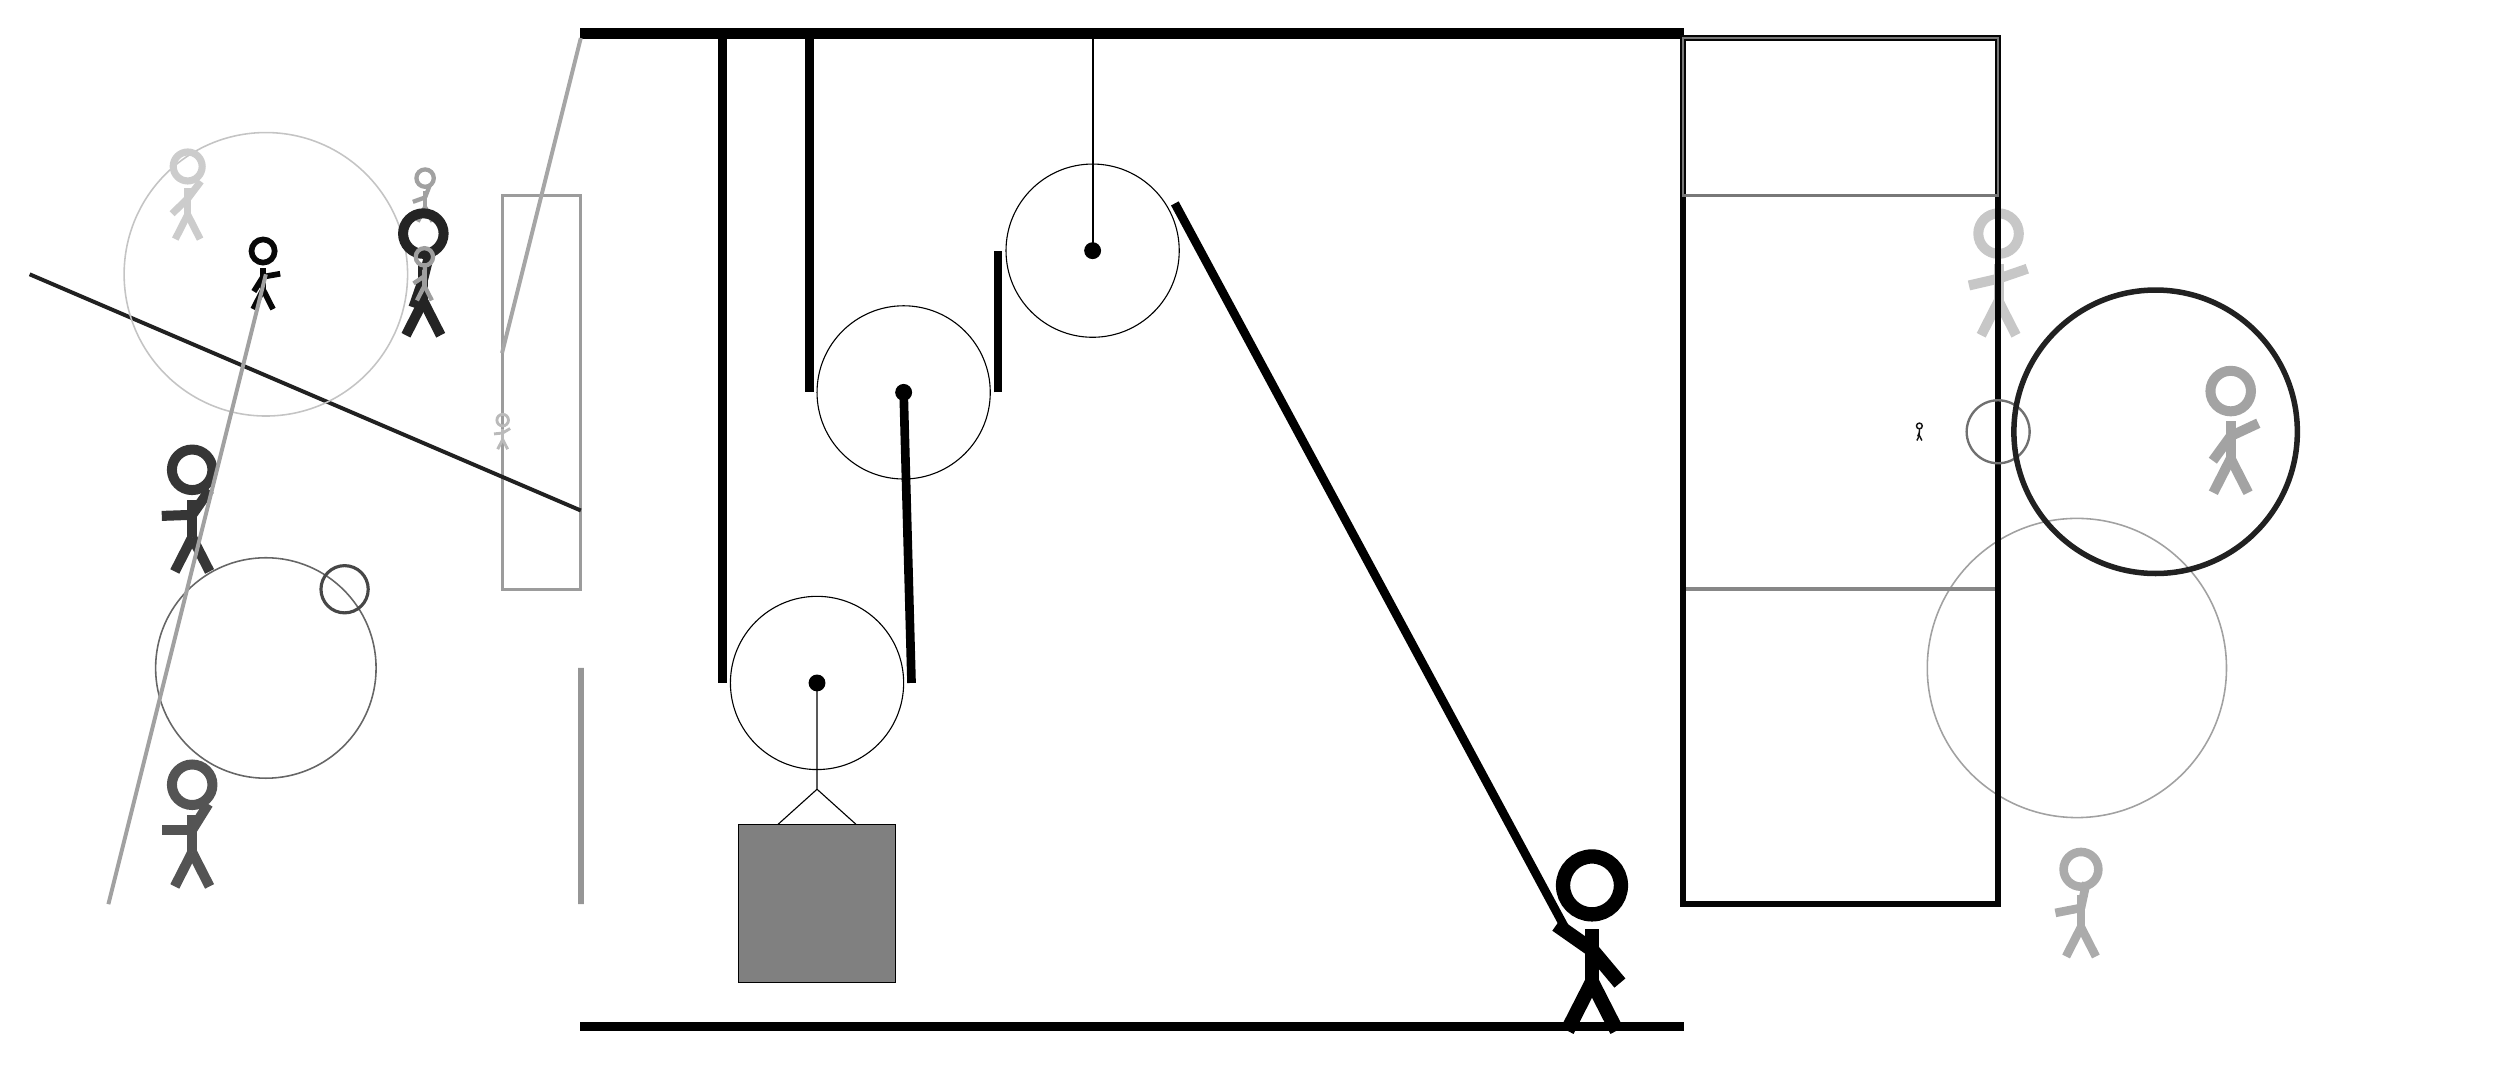
\begin{tikzpicture}
			%%%%% START %%%%%
			
			\draw[fill=black] (-2, 9) rectangle (12, 9.125);
			
			\node[line width=0.2mm, color=black!36] at (19, 4) {\Strichmaxerl[7][54][25]};
			
			\node[line width=0.5mm, color=black!37] at (-4, 7) {\Strichmaxerl[3][20][69]};
			\draw[line width=0.4mm, color=black!39] (-2, 2) rectangle (-3, 7);
			\node[line width=0.2mm, color=black!79] at (-7, 3) {\Strichmaxerl[7][2][55]};
			
			\node[line width=0.2mm, color=black!22] at (16, 6) {\Strichmaxerl[7][13][19]};
			
			\draw[line width=0.5mm, color=black!87](-2, 3) -- (-9, 6);
			\draw [line width=0.2mm, color=black!60](-6, 1) circle (1.4);
			\node[line width=0.3mm, color=black!97] at (-6, 6) {\Strichmaxerl[4][58][10]};
			\draw [line width=0.2mm, color=black!37](17, 1) circle (1.9);
			
			\draw[line width=0.5mm, color=black!47](12, 2) -- (16, 2);
			\draw[line width=0.7mm, color=black!41] (-2, 1) rectangle (-2, -2);
			
			\draw[line width=0.4mm, color=black!75] (14, 9) rectangle (16, 9);
			\draw[line width=0.2mm, color=black!47] (12, 7) rectangle (16, 7);
			
			\draw [line width=0.2mm, color=black!23](-6, 6) circle (1.8);
			\node[line width=0.5mm, color=black!27] at (-3, 4) {\Strichmaxerl[2][6][31]};
			\node[line width=0.7mm, color=black!20] at (-7, 7) {\Strichmaxerl[5][44][53]};
			\draw[line width=0.7mm, color=black!98] (12, 9) rectangle (16, -2);
			\draw [line width=0.3mm, color=black!56](16, 4) circle (0.4);
			\draw [line width=0.7mm, color=black!87](18, 4) circle (1.8);
			\draw [line width=0.4mm, color=black!96](22, 4) circle (0.0);
			\node[line width=0.4mm, color=black!86] at (-4, 6) {\Strichmaxerl[7][71][76]};
			
			\draw[line width=0.3mm, color=black!53] (12, 7) rectangle (16, 9);
			\node[line width=0.5mm, color=black!67] at (-7, -1) {\Strichmaxerl[7][0][58]};
			\draw[line width=0.5mm, color=black!35](-3, 5) -- (-2, 9);
			\node[line width=0.7mm, color=black!38] at (-4, 6) {\Strichmaxerl[3][34][86]};
			
			\draw [line width=0.4mm, color=black!72](-5, 2) circle (0.3);
			\draw[line width=0.5mm, color=black!37](-6, 6) -- (-8, -2);
			\node[line width=0.2mm, color=black!93] at (15, 4) {\Strichmaxerl[1][67][88]};
			\node[line width=0.6mm, color=black!33] at (17, -2) {\Strichmaxerl[6][11][78]};
			
			
			\draw (1, 0.81) circle (1.1);
			\draw[fill=black] (1, 0.81) circle (0.1);
			
			\draw (2.1, 4.5) circle (1.1);
			\draw[fill=black] (2.1, 4.5) circle (0.1);
			
			\draw (4.5, 6.3) circle (1.1);
			\draw[fill=black] (4.5, 6.3) circle (0.1);
			\draw[thick] (4.5, 6.3) -- (4.5, 9);
			
			\draw (1, 0.81) -- (1, -0.54) -- (0.5, -0.99) -- (1.5, -0.99) -- (1, -0.54);
			\draw[fill=black!50] (0, -0.99) rectangle (2, -2.99);
			
			\draw[line width=1.1mm] (-0.2, 9) -- (-0.2, 0.81);
			\centerarc[line width=1.1mm](1, 0.81)(180:360:1.2000000000000002);
			\draw[line width=1.1mm](2.2, 0.81) -- (2.1, 4.5);
			\draw[line width=1.1mm] (0.9, 9) -- (0.9, 4.5);
			\centerarc[line width=1.1mm](2.1, 4.5)(180:360:1.2000000000000002);
			\draw[line width=1.1mm](3.3, 4.5) -- (3.3, 6.3);
			\centerarc[line width=1.1mm](4.5, 6.3)(30:180:1.2000000000000002);
			\draw[line width=1.1mm] (5.544, 6.9) -- (10.5, -2.3);
			
			\node at (10.8, -2.5) {\Strichmaxerl[10][-35][-50]};
			
			\draw[fill=black] (-2, -3.5) rectangle (12, -3.6);
			
			%%%%% END %%%%%
		\end{tikzpicture}
	\end{figure}	
\end{document}